\documentclass[
11pt, % The default document font size, options: 10pt, 11pt, 12pt
%codirector, % Uncomment to add a codirector to the title page
]{charter} 




% El títulos de la memoria, se usa en la carátula y se puede usar el cualquier lugar del documento con el comando \ttitle
\titulo{Diseño e implementación de un data logger para mediciones meteorológicas} 

% Nombre del posgrado, se usa en la carátula y se puede usar el cualquier lugar del documento con el comando \degreename
\posgrado{Carrera de Especialización en Sistemas Embebidos} 
%\posgrado{Carrera de Especialización en Internet de las Cosas} 
%\posgrado{Carrera de Especialización en Intelegencia Artificial}
%\posgrado{Maestría en Sistemas Embebidos} 
%\posgrado{Maestría en Internet de las cosas}

% Tu nombre, se puede usar el cualquier lugar del documento con el comando \authorname
\autor{Ing. Renato Barresi} 

% El nombre del director y co-director, se puede usar el cualquier lugar del documento con el comando \supname y \cosupname y \pertesupname y \pertecosupname
\director{Esp. Lic. Pablo Zizzutti}
\pertenenciaDirector{FIUBA} 
% FIXME:NO IMPLEMENTADO EL CODIRECTOR ni su pertenencia
\codirector{} % para que aparezca en la portada se debe descomentar la opción codirector en el documentclass
\pertenenciaCoDirector{}

% Nombre del cliente, quien va a aprobar los resultados del proyecto, se puede usar con el comando \clientename y \empclientename
\cliente{Javier Marin}
\empresaCliente{Tech Enterprise S.A}

% Nombre y pertenencia de los jurados, se pueden usar el cualquier lugar del documento con el comando \jurunoname, \jurdosname y \jurtresname y \perteunoname, \pertedosname y \pertetresname.
\juradoUno{Nombre y Apellido (1)}
\pertenenciaJurUno{pertenencia (1)} 
\juradoDos{Nombre y Apellido (2)}
\pertenenciaJurDos{pertenencia (2)}
\juradoTres{Nombre y Apellido (3)}
\pertenenciaJurTres{pertenencia (3)}
 
\fechaINICIO{01 de marzo de 2022}		%Fecha de inicio de la cursada de GdP \fechaInicioName
\fechaFINALPlan{19 de abril de 2022} 	%Fecha de final de cursada de GdP
\fechaFINALTrabajo{15 de mayo de 2022}	%Fecha de defensa pública del trabajo final


\begin{document}

\maketitle
\thispagestyle{empty}
\pagebreak


\thispagestyle{empty}
{\setlength{\parskip}{0pt}
\tableofcontents{}
}
\pagebreak


\section*{Registros de cambios}
\label{sec:registro}


\begin{table}[ht]
\label{tab:registro}
\centering
\begin{tabularx}{\linewidth}{@{}|c|X|c|@{}}
\hline
\rowcolor[HTML]{C0C0C0} 
Revisión & \multicolumn{1}{c|}{\cellcolor[HTML]{C0C0C0}Detalles de los cambios realizados} & Fecha      \\ \hline
0      & Creación del documento                                 &\fechaInicioName \\ \hline
1      & Se completa hasta el punto 5 inclusive                 & 15/03/2022 \\ \hline
2      & Se completa hasta el punto 9 inclusive y agregan correcciones & 27/03/2022\\ \hline
\end{tabularx}
\end{table}

\pagebreak



\section*{Acta de constitución del proyecto}
\label{sec:acta}

\begin{flushright}
Buenos Aires, \fechaInicioName
\end{flushright}

\vspace{2cm}

Por medio de la presente se acuerda con el Ing. \authorname\hspace{1px} que su Trabajo Final de la \degreename\hspace{1px} se titulará ``\ttitle'', consistirá esencialmente en la implementación de un prototipo de computador que hará de interfaz con sensores meteorológicos y el internet, y tendrá un presupuesto preliminar estimado de 600 hs de trabajo y \$ 1000 US, con fecha de inicio \fechaInicioName\hspace{1px} y fecha de presentación pública \fechaFinalName.

Se adjunta a esta acta la planificación inicial.

\vfill

% Esta parte se construye sola con la información que hayan cargado en el preámbulo del documento y no debe modificarla
\begin{table}[ht]
\centering
\begin{tabular}{ccc}
\begin{tabular}[c]{@{}c@{}}Ariel Lutenberg \\ Director posgrado FIUBA\end{tabular} & \hspace{2cm} & \begin{tabular}[c]{@{}c@{}}\clientename \\ \empclientename \end{tabular} \vspace{2.5cm} \\ 
\multicolumn{3}{c}{\begin{tabular}[c]{@{}c@{}} \supname \\ Director del Trabajo Final\end{tabular}} \vspace{2.5cm} \\
%\begin{tabular}[c]{@{}c@{}}\jurunoname \\ Jurado del Trabajo Final\end{tabular}     &  & \begin{tabular}[c]{@{}c@{}}\jurdosname\\ Jurado del Trabajo Final\end{tabular}  \vspace{2.5cm}  \\
%\multicolumn{3}{c}{\begin{tabular}[c]{@{}c@{}} \jurtresname\\ Jurado del Trabajo Final\end{tabular}} \vspace{.5cm}                                                                     
\end{tabular}
\end{table}




\section{1. Descripción técnica-conceptual del proyecto a realizar}
\label{sec:descripcion}

El cambio climático es una de las mayores problemáticas que enfrenta la humanidad en el siglo 21, se estima que 800 millones de personas son vulnerables a los efectos negativos que puede generar este, es por eso que se deben generar políticas enfocadas a luchar y contrarrestar los perjuicios que pueden ser causados por el cambio climático. Estas políticas deben estar basadas en datos y mediciones científicas, las cuales se obtienen en gran parte por medio de estaciones meteorológicas automáticas.   

Una estación meteorológica automática se encarga de tomar mediciones meteorológicas, procesarlas, guardarlas y transmitirlas. El elemento principal de esta es un data logger, que es un computador con distintos periféricos para cumplir las funciones requeridas por la estación. 

En Paraguay, el mercado de estaciones meteorológicas automáticas esta dominado por productos del extranjero, las que tienen costo muy elevado para el presupuesto que manejan las entidades publicas y privadas, también, el bajo nivel de customización que ofrecen, es un impedimento para poder modificar a la estación en base a las posibilidades del cliente.

Actualmente, Tech Enterpise S.A cuenta con data loggers propios, basados en microcontroladores de 8 bits, como el atmega328p y atmega2560. La baja cantidad de periféricos, velocidad, memoria RAM y FLASH con los que cuentan estos microcontroladores, limita las funcionalidades y escalabilidad del código del data logger. Es por esto que la empresa busca migrar a microcontroladores de 32 bits, como el STM32F767ZI, que cuenta con una frecuencia máxima de 216 MHz, memoria FLASH de 2 Mbytes y memoria SRAM de 512 Kbytes. También, cuenta con interfaz MAC que permite utilizar integrados PHY para Ethernet.   

En lo que respecta al presente trabajo, se propone diseñar una solución basada en el mencionado microcontrolador, que sea capaz de comunicarse con sensores utilizando el protocolo de comunicación SDI-12, con una memoria FLASH y memoria SD y que pueda transmitir la información por medio de protocolos de capa 2 como el PPP y Ethernet.

En la figura 1 se muestra el diagrama en bloques del sistema. El microcontrolador se encarga de comunicarse con distintos periféricos, como la memoria SD, memoria Flash, ADC, etc. Además de poder comunicarse con dichos componentes, debe de ser capaz de actuar como cliente FTP.

%\vspace{25px}

\begin{figure}[htpb]
\centering 
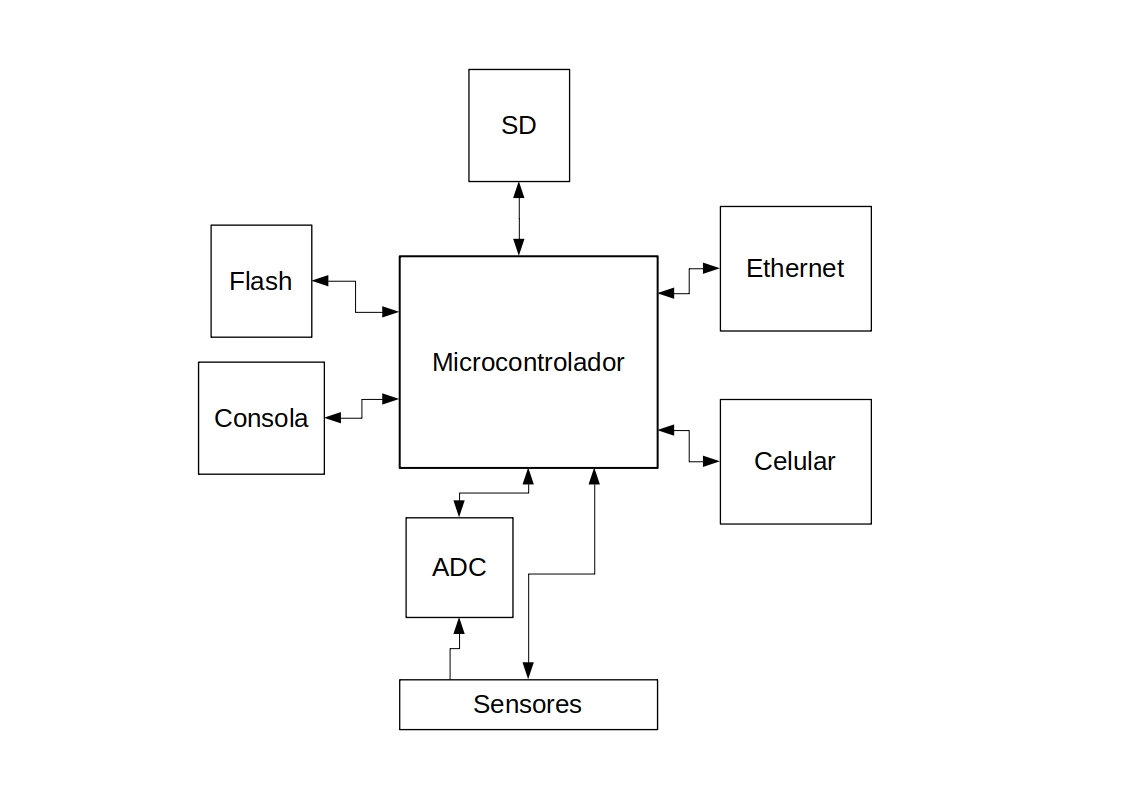
\includegraphics[width=.9\textwidth]{./Figuras/Diagrama_de_bloques_modulos.jpg}
\caption{Diagrama en bloques del sistema.}
\label{fig:diagBloques}
\end{figure}

\vspace{25px}



\section{2. Identificación y análisis de los interesados}
\label{sec:interesados}

\begin{table}[ht]
%\caption{Identificación de los interesados}
%\label{tab:interesados}
\begin{tabularx}{\linewidth}{@{}|l|X|X|l|@{}}
\hline
\rowcolor[HTML]{C0C0C0} 
Rol           & Nombre y Apellido & Organización 	& Puesto 	\\ \hline
Auspiciante   &     Jose Flecha              &     Data system S.A         	&       Director ejecutivo  	\\ \hline
Cliente       & \clientename      &\empclientename	& Director ejecutivo       	\\ \hline
Impulsor      & Julio Mendez    &  CONACYT    	&  Director PROINOVA    	\\ \hline
Responsable   & \authorname       & FIUBA        	& Alumno 	\\ \hline
Orientador    & \supname	      & \pertesupname 	& Director Trabajo final \\ \hline
Opositores    &        Jack  Johnson          &      Campbell Scientific        	&   Sales manager     	\\ \hline
Usuario final & Fernando Pio Barrios   & Dirección de Meteorología e Hidrología              	& Director       	\\ \hline
\end{tabularx}
\end{table}


\section{3. Propósito del proyecto}
\label{sec:proposito}

El propósito de este proyecto es diseñar e implementar el prototipo de un data logger basado en un microcontrolador de 32 bits que permita comunicarse con sensores meteorológicos, procesar los datos, almacenar la información a una memoria SD y trasmitir a un servidor FTP.

\section{4. Alcance del proyecto}
\label{sec:alcance}

El proyecto incluye los siguientes puntos:
\begin{itemize}
\item Diseño, programación e implementación de un sistema embebido que sea capaz de comunicarse con distintos sensores, procesar los datos, guardar y transmitirlos por internet.
\item Diseño de una biblioteca modular en C, que permita comunicarse con sensores que utilizan el protocolo SDI-12.
\item Diseño de una biblioteca modular en C, que permita comunicarse con memorias de tipo FLASH.
\item Diseño de la arquitectura del sistema embebido.
\item Prototipo en protoboard del sistema embebido.
\item Diseño de la placa de circuito impreso.
\item Verificación funcional de la placa de circuito impreso.
\end{itemize}

Queda excluido del alcance del proyecto:
\begin{itemize}
\item Desarrollo de un cargador solar.
\item Diseño de un RTOS.
\item Diseño de un stack TCP/IP.
\item Testeo de más de una semana del sistema.
\item Testeo de rangos de temperatura y humedad mínimos y máximos.
\end{itemize}


\section{5. Supuestos del proyecto}
\label{sec:supuestos}


Para el desarrollo del presente proyecto se supone que: 

\begin{itemize}
	\item Se contará con una placa NUCLEO-F767ZI.
	\item Se podrá contar con los insumos necesarios en tiempo y forma.
	\item Se contará con las instalaciones disponibles para las pruebas pertinentes.
	\item Se dispondrá del tiempo necesario para el desarrollo del proyecto.
	\item Se contará con sensores meteorológicos para realizar las mediciones.
	\item Se contará con un módem celular para conexiones GPRS/GSM.
	\item Se cuenta con toda la información técnica de sensores meteorológicos, módem, microcontroladores, Ethernet, etc.
\end{itemize}

\section{6. Requerimientos}
\label{sec:requerimientos}

\begin{enumerate}
	\item Requerimientos de firmware.
		\begin{enumerate}
			\item El proyecto sera desarrollado y mantenido mediante el control de versiones GIT. 
			\item El proyecto sera desarrollado en lenguaje C, compilado con ARM GCC.
			\item Se deberá de desarrollar biblioteca de control del conversor analógico digital.
			\item Se deberá de desarrollar biblioteca de control de la memoria FLASH. 
			\item Se deberá de desarrollar biblioteca del protocolo SDI-12.
		\end{enumerate}
	\item Requerimientos de documentación.
		\begin{enumerate}
			\item El código será documentado con la herramienta Doxygen.
			\item El ciclo de vida del proyecto sera respaldado por una memoria técnica.
			\item Se entregaran informes de avance.
		\end{enumerate}
	\item Requerimientos asociados con la arquitectura del sistema.
		\begin{enumerate}
		\item El data logger se debe basar en el STM32F767ZI.
		\item El STM32F767ZI se debe comunicar con una memoria FLASH por medio del protocolo SPI.
		\item El STM32F767ZI se debe comunicar con una memoria SD, por medio del protocolo SPI.
		\item El STM32F767ZI se debe comunicar con un conversor analógico digital, por medio del protocolo I2C.
		\end{enumerate}
	\item Requerimientos de la interfaz.
		\begin{enumerate}
		\item El sistema debe contar con protección contra cortocircuitos, sobre voltaje y bajo voltaje. 
		\item El sistema debe funcionar con un rango de tension entre 7V y 24 VDC.
		\item El sistema debe contar con dos puertos RS-232.
		\item El sistema debe contar con un puerto Ethernet.
		\item El sistema debe contar con una interfaz SD.
		\item El sistema debe contar con un puerto micro USB.
		\item El sistema debe contar con borneras para conexión con los sensores.
		\end{enumerate}
\end{enumerate}


\section{7. Historias de usuarios (\textit{Product backlog})}
\label{sec:backlog}

Roles: 
\begin{itemize}
	\item Usuario/a - Persona que hará uso de la información proveniente de la estación.
	\item Instalador/a - Es la persona encargada del ensamblaje y puesta en marcha de la estación de Tech Enterprise S.A. A su cargo se encuentra el diseño y ensamblado de la estación para el usuario, esto es, elegir los sensores en función a las necesidades del usuario, tipo de alimentación, forma de conexión con la red, etc.   
	\item Cliente - Es la persona que auspiciara el proyecto de la estación.
\end{itemize}

Ponderación:
	\begin{itemize}
		\item Este puntaje esta dado por la relevancia que tiene la historia de usuario para el éxito del proyecto definido en esta planificación.
		\item Se utilizará una escala de prioridad de 1, 2, y 4 puntos para las historias.
		\begin{itemize}
			\item Dificultad/tiempo.
			\item Complejidad
			\item Incertidumbre/Riesgo.

		\end{itemize}
	\end{itemize}
Historias de usuario:
	\begin{itemize}
	\item Como ingeniero agrónomo, quiero poder utilizar los sensores que utilicen el protocolo SDI-12.
		\begin{itemize}
			\item Dificultad/tiempo: 2.
			\item Complejidad: 2.
			\item Incertidumbre/Riesgo: 1.
			\item Total: 5 pts.
		\end{itemize}
	\item Como instalador, deseo poder actualizar el software de la estación de forma remota, subiendo el archivo binario al servidor FTP (4p).
		\begin{itemize}
			\item Dificultad/tiempo: 4.
			\item Complejidad: 4.
			\item Incertidumbre/Riesgo: 4.
			\item Total: 12 pts.
		\end{itemize}
	\item Como meteorólogo, quiero poder recibir la información en un archivo .txt (4p).
		\begin{itemize}
			\item Dificultad/tiempo: 1.
			\item Complejidad: 1.
			\item Incertidumbre/Riesgo: 1.
			\item Total: 3 pts.
		\end{itemize}
	\item Como project mánager deseo poder utilizar el protocolo Ethernet para realizar conexiones a internet. 
		\begin{itemize}
			\item Dificultad/tiempo: 2.
			\item Complejidad: 4.
			\item Incertidumbre/Riesgo: 1.
			\item Total: 7 pts.
		\end{itemize}
	\end{itemize}

\section{8. Entregables principales del proyecto}
\label{sec:entregables}

\begin{itemize}
	\item Informe final.
	\item Manual de configuración y puesta en marcha.
	\item Diagrama de circuitos esquemáticos.
	\item Código fuente del firmware.
	\item Informe de avance. 
\end{itemize}


\section{9. Desglose del trabajo en tareas}
\label{sec:wbs}

\begin{enumerate}
\item Planificación del proyecto (40hs)
	\begin{enumerate}
	\item Realizar el plan de proyecto (20 hs).
	\item Redactar requisitos del firmware (20 hs).
	\end{enumerate}
\item Investigación preliminar (40 hs)
	\begin{enumerate}
	\item Investigar características técnicas de cada uno de los componentes a utilizar (16 hs).
	\item Investigar bibliotecas TCP/IP (12 hs).
	\item Investigar sobre sistemas operativos de tiempo real (12 hs).
	\end{enumerate}
\item Desarrollo de firmware (300 hs)
	\begin{enumerate}
	\item Configuración inicial del microcontrolador y sus distintos periféricos (20 hs). 
	\item Diseñar algoritmo de configuración de la estación (30 hs).
	\item Diseñar biblioteca para control de memoria FLASH (40 hs).
	\item Integrar biblioteca para control de memoria SD (10 hs).
	\item Diseñar biblioteca para comunicación por medio del protocolo SDI-12 (40 hs).
	\item Diseñar biblioteca para control del conversor analógico digital (40 hs).
	\item Diseñar biblioteca para cliente FTP (40 hs).
	\item Integración de las distintas bibliotecas (40 hs).
	\item Diseñar máquina de estados finitos (40 hs).
	\end{enumerate}
\item Validación (80 hs).
	\begin{enumerate}
	\item Ejecutar esquema de pruebas de conexión PPP (20 hs).
	\item Ejecutar esquema de pruebas de conexión Ethernet (20 hs).
	\item Ejecutar esquema de pruebas de guardado en memoria SD (10 hs).
	\item Ejecutar esquema de pruebas de protocolo SDI-12 (5 hs).
	\item Ejecutar esquema de pruebas de cliente FTP (25 hs).

	\end{enumerate}
\item Documentación (30 hs).
	\begin{enumerate}
	\item Documentación HTML con Doxygen (5 hs).
	\item Redacción de informes de avance (25 hs).
	
	\end{enumerate}
\item Elaboración final (110 hs).
	\begin{enumerate}
	\item Redacción del manuscrito final (40 hs).
	\item Elaboración de la memoria técnica (40 hs).
	\item Preparación de la exposición del trabajo final (20 hs).	
	\item Ensayo de la exposición (10 hs).
	\end{enumerate}
\end{enumerate}

Cantidad total de horas: (600 hs).

\section{10. Diagrama de Activity On Node}
\label{sec:AoN}


\begin{figure}[htpb]
\centering 
\includegraphics[width=1.35\textwidth]{./Figuras/diagramaAoN.jpg}
\caption{Diagrama en \textit{Activity on Node}}
\label{fig:AoN}
\end{figure}

\section{11. Diagrama de Gantt}
\label{sec:gantt}

\begin{consigna}{red}

Existen muchos programas y recursos \textit{online} para hacer diagramas de gantt, entre los cuales destacamos:

\begin{itemize}
\item Planner
\item GanttProject
\item Trello + \textit{plugins}. En el siguiente link hay un tutorial oficial: \\ \url{https://blog.trello.com/es/diagrama-de-gantt-de-un-proyecto}
\item Creately, herramienta online colaborativa. \\\url{https://creately.com/diagram/example/ieb3p3ml/LaTeX}
\item Se puede hacer en latex con el paquete \textit{pgfgantt}\\ \url{http://ctan.dcc.uchile.cl/graphics/pgf/contrib/pgfgantt/pgfgantt.pdf}
\end{itemize}

Pegar acá una captura de pantalla del diagrama de Gantt, cuidando que la letra sea suficientemente grande como para ser legible. 
Si el diagrama queda demasiado ancho, se puede pegar primero la ``tabla'' del Gantt y luego pegar la parte del diagrama de barras del diagrama de Gantt.

Configurar el software para que en la parte de la tabla muestre los códigos del EDT (WBS).\\
Configurar el software para que al lado de cada barra muestre el nombre de cada tarea.\\
Revisar que la fecha de finalización coincida con lo indicado en el Acta Constitutiva.

En la figura \ref{fig:gantt}, se muestra un ejemplo de diagrama de gantt realizado con el paquete de \textit{pgfgantt}. En la plantilla pueden ver el código que lo genera y usarlo de base para construir el propio.

\begin{figure}[htbp]
\begin{center}
\begin{ganttchart}{1}{12}
  \gantttitle{2020}{12} \\
  \gantttitlelist{1,...,12}{1} \\
  \ganttgroup{Group 1}{1}{7} \\
  \ganttbar{Task 1}{1}{2} \\
  \ganttlinkedbar{Task 2}{3}{7} \ganttnewline
  \ganttmilestone{Milestone o hito}{7} \ganttnewline
  \ganttbar{Final Task}{8}{12}
  \ganttlink{elem2}{elem3}
  \ganttlink{elem3}{elem4}
\end{ganttchart}
\end{center}
\caption{Diagrama de gantt de ejemplo}
\label{fig:gantt}
\end{figure}


\begin{landscape}
\begin{figure}[htpb]
\centering 
\includegraphics[height=.85\textheight]{./Figuras/Gantt-2.png}
\caption{Ejemplo de diagrama de Gantt rotado}
\label{fig:diagGantt}
\end{figure}

\end{landscape}

\end{consigna}


\section{12. Presupuesto detallado del proyecto}
\label{sec:presupuesto}
\begin{table}[htpb]
\centering
\begin{tabularx}{\linewidth}{@{}|X|c|r|r|@{}}
\hline
\rowcolor[HTML]{C0C0C0} 
\multicolumn{4}{|c|}{\cellcolor[HTML]{C0C0C0}COSTOS DIRECTOS} \\ \hline
\rowcolor[HTML]{C0C0C0} 
Descripción & 
  \multicolumn{1}{c|}{\cellcolor[HTML]{C0C0C0}Cantidad} &
  \multicolumn{1}{c|}{\cellcolor[HTML]{C0C0C0}Valor unitario} &
  \multicolumn{1}{c|}{\cellcolor[HTML]{C0C0C0}Valor total} \\ \hline
Mano de obra &
  \multicolumn{1}{c|}{600} &
  \multicolumn{1}{c|}{\$ 5} &
  \multicolumn{1}{c|}{\$ 3000} \\ \hline

Placa Nucleo &
  \multicolumn{1}{c|}{1} &
  \multicolumn{1}{c|}{\$ 60} &
  \multicolumn{1}{c|}{\$ 60} \\ \hline
Modem celular &
  \multicolumn{1}{c|}{1} &
  \multicolumn{1}{c|}{\$ 90} &
  \multicolumn{1}{c|}{\$ 90} \\ \hline
Memoria SD &
  \multicolumn{1}{c|}{1} &
  \multicolumn{1}{c|}{\$ 15} &
  \multicolumn{1}{c|}{\$ 15} \\ \hline
Memoria Flash &
  \multicolumn{1}{c|}{1} &
  \multicolumn{1}{c|}{\$ 5} &
  \multicolumn{1}{c|}{\$ 5} \\ \hline
Conversor analogico digital &
  \multicolumn{1}{c|}{1} &
  \multicolumn{1}{c|}{\$ 20} &
  \multicolumn{1}{c|}{\$ 20} \\ \hline
Sensor de suelo &
  \multicolumn{1}{c|}{1} &
  \multicolumn{1}{c|}{\$ 200} &
  \multicolumn{1}{c|}{\$ 200} \\ \hline
Sensor de corriente &
  \multicolumn{1}{c|}{1} &
  \multicolumn{1}{c|}{\$ 24} &
  \multicolumn{1}{c|}{\$ 24} \\ \hline
\multicolumn{3}{|c|}{SUBTOTAL} & 
  \multicolumn{1}{c|}{\$ 3414} \\ \hline
\rowcolor[HTML]{C0C0C0} 
\multicolumn{4}{|c|}{\cellcolor[HTML]{C0C0C0}COSTOS INDIRECTOS} \\ \hline
\rowcolor[HTML]{C0C0C0} 
Descripción &
  \multicolumn{1}{c|}{\cellcolor[HTML]{C0C0C0}Cantidad} &
  \multicolumn{1}{c|}{\cellcolor[HTML]{C0C0C0}Valor unitario} &
  \multicolumn{1}{c|}{\cellcolor[HTML]{C0C0C0}Valor total} \\ \hline
\multicolumn{1}{|l|}{ Insumos varios} &
  \multicolumn{1}{c|}{1} &
  \multicolumn{1}{c|}{\$ 3000} &
  \multicolumn{1}{c|}{\$ 3000} \\ \hline
\multicolumn{3}{|c|}{SUBTOTAL} &
  \multicolumn{1}{c|}{\$ 3000} \\ \hline
\rowcolor[HTML]{C0C0C0}
\multicolumn{3}{|c|}{TOTAL} & \$ 6414
   \\ \hline
\end{tabularx}%
\end{table}


\section{13. Gestión de riesgos}
\label{sec:riesgos}


a) Identificación de los riesgos y estimación de sus consecuencias:
 
Riesgo 1: La placa nucleo-F767ZI deja de funcionar.
\begin{itemize}
	\item Severidad (S): 8\\
	La severidad es moderada/alta, debido a que si la placa deja de funcionar demoraría en el inicio de la implementación del firmware.
	\item Ocurrencia (0): 2\\
	 La probabilidad es baja, ademas se cuenta con una placa de repuesto. 
\end{itemize}   
Riesgo 2: No se cuenta con un módem celular. 
\begin{itemize}
	\item Severidad (S): 5 \\
	La severidad es moderada, debido a que se requiere a un módem celular para poder desarrollar la implementación de los módulos dependientes de este.
	\item Ocurrencia (O): 1 \\
	La probabilidad es baja, debido a que se cuenta con disponibilidad del modem.
\end{itemize}

Riesgo 3: Imposibilidad de cumplir los plazos planteados.
\begin{itemize}
	\item Severidad (S): 7 \\
	La severidad es moderada, algunos requisitos podrían requerir tiempos mas amplios de implementación que los presentados en el proyecto.
	\item Ocurrencia (O): 4 \\
	La probabilidad es moderada/baja, debido a que existe una planificación de previa.
\end{itemize}

Riesgo 4: Escasez del hardware en el mercado.
\begin{itemize}
	\item Severidad (S): 8 \\
	La severidad es alta, esto seria un impedimento para el desarrollo de distintos módulos del proyecto.
	\item Ocurrencia (O): 4 \\
	La probabilidad es moderada/baja, debido a que el hardware seleccionado es accesible en el mercado.
\end{itemize}

Riesgo 5: Conexión al internet es de baja calidad.
\begin{itemize}
	\item Severidad (S): 6 \\
	La severidad es moderada, debido a que es un requerimiento principal del sistema.
	\item Ocurrencia (O): 4 \\
	La probabilidad es moderada/baja, debido a que el stack a utilizar esta bien establecido.
\end{itemize}

b) Tabla de gestión de riesgos:      (El RPN se calcula como RPN=SxO)

\begin{table}[htpb]
\centering
\begin{tabularx}{\linewidth}{@{}|X|c|c|c|c|c|c|@{}}
\hline
\rowcolor[HTML]{C0C0C0} 
Riesgo & S & O & RPN & S* & O* & RPN* \\ \hline
La placa nucleo-F767ZI deja de funcionar       &  8 &  2 &  16   &    &    &      \\ \hline
No se cuenta con un modem celular       & 5  & 1  &  5   &    &    &      \\ \hline
Imposibilidad de cumplir los plazos planteados       &  7 & 4  &  28   &  6  & 3    &   18   \\ \hline
Escasez del hardware en el mercado       &  8 & 4  &  32  &  7  & 2   &  14    \\ \hline
Conexión al internet es de baja calidad       & 6  & 4  &  24   &  5  &  2  &     10 \\ \hline
\end{tabularx}%
\end{table}

Criterio adoptado: 
Se tomarán medidas de mitigación en los riesgos cuyos números de RPN sean mayores a 20

Nota: los valores marcados con (*) en la tabla corresponden luego de haber aplicado la mitigación.

c) Plan de mitigación de los riesgos que originalmente excedían el RPN máximo establecido:
 
Riesgo 3: Imposibilidad de cumplir los plazos planteados
\begin{itemize}
	\item Plan de mitigación: Re asignación de horas atrasadas y rigurosidad con el cumplimiento.
	\item Severidad (6): La severidad es moderada, algunos requisitos podrían requerir tiempos mas amplios de implementación que los presentados en el proyecto.
	\item Ocurrencia (3): La probabilidad es baja, debido a que existe una planificación de previa, y rigurosidad con el cumplimiento de estas.
\end{itemize}

Riesgo 4: Escasez del hardware en el mercado
\begin{itemize}
	\item Plan de mitigación: Compra de componentes lo antes posible.
	\item Severidad (7): La severidad es moderada, esto seria un impedimento para el desarrollo de distintos módulos del proyecto.
	\item Ocurrencia (2): La probabilidad es baja, debido a que el hardware seleccionado es accesible en el mercado y se comprara con anticipación a los componentes necesarios.
\end{itemize}

Riesgo 5: Conexión al internet es de baja calidad
\begin{itemize}
	\item Plan de mitigación: Se realizaran los estudios correspondientes con antelación para la correcta configuración del stack.
	\item Severidad (5): La severidad es moderada, debido a que es un requerimiento principal del sistema.
	\item Ocurrencia (2): La probabilidad es baja, debido a que el stack a utilizar esta bien establecido y se estudiará con tiempo la documentación.
\end{itemize}



\section{14. Gestión de la calidad}
\label{sec:calidad}
\begin{itemize}
\item Requerimiento 1.1: Se deberá de poder denir la fecha y horario del sistema, utilizando el RTC.
	\begin{itemize}
		\item Verificación: Se implementara un menu de configuracion donde el usuario podra configurar al RTC.
		\item Validación: Se leera el horario del RTC.
	\end{itemize}
\item Requerimiento 1.2: Se deberá de poder denir el periodo de transmisión de los archivos al servidor.
	\begin{itemize}
		\item Verificación: Se implementara un menu de configuracion donde el usuario podra definir el periodo de transmision.
		\item Validación: Se verificara si la transmision se realiza en el periodo establecido.
	\end{itemize}
\item Requerimiento 1.3: Se deberá de poder denir el periodo de la toma de muestras de los sensores.
	\begin{itemize}
		\item Verificación: Se implementara un menu de configuracion donde el usuario podra definir el periodo de muestreo de los sensores.
		\item Validación: La comunicacion con los sensores debe de ser la que el usuario definio.
	\end{itemize}
\item Requerimiento 1.4: Se deberá de poder defir el nombre particular de la estación.
	\begin{itemize}
		\item Verificación: Se implementara un menu de configuracion donde el usuario podra definir el nombre de la estacion.
		\item Validación: El nombre de los archivos enviados al servidor deben de contener el nombre definido por el usuario.
	\end{itemize}
\item Requerimiento 1.5: Se deberá de poder seleccionar los sensores conectados.
	\begin{itemize}
		\item Verificación: Se implementara un menu de configuracion donde el usuario podra definir que sensores estan conectados al data logger.
		\item Validación: El data logger debera de comunicarse con los sensores seleccionados por el usuario.
	\end{itemize}
\item Requerimiento 1.6: Se podrá denir el tipo de conexión para la red.
	\begin{itemize}
		\item Verificación: Se implementara un menu de configuracion donde el usuario podra definir que tipo de conexion de red cuenta el data logger.
		\item Validación: La conexion a internet debe de darse por medio de la conexion definida por el usuario. 
	\end{itemize}
\item Requerimiento 2.1: El software deberá de poder comunicarse con sensores que utilicen el protocolo SDI-12.
	\begin{itemize}
		\item Verificación: Se implementara una biblioteca para el manejo de comunicaciones por el protocolo SDI-12
		\item Validación: El data logger debera de ser capaz de obtener datos de un sensor SDI-12.
	\end{itemize}
\item Requerimiento 2.2: El software deberá de poder adquirir datos de sensores analógicos.
	\begin{itemize}
		\item Verificación: Se implementara una biblioteca para el manejo de comunicacion con el ADS1115 por medio del protocolo I2C.
		\item Validación: El microcontrolador debera de ser capaz de comunicarse con el ADS1115 y obtener datos de un sensor de corriente.
	\end{itemize}	
\item Requerimiento 2.3: El sofware deberá de poder poner al microcontrolador entrar en modo de bajo consumo.
	\begin{itemize}
		\item Verificación: Se implementara un modulo que permita entrar y salir al microcontrolador de modo de bajo consumo. 
		\item Validación: Luego de realizar la transmision al servidor, el microcontrolador debe de entrar en modo de bajo consumo.
	\end{itemize}
\item Requerimiento 3.1: El software podrá detectar si la memoria SD esta conectada o no.
	\begin{itemize}
		\item Verificación: Se implementara la logica de deteccion de la conexion con la memoria SD.
		\item Validación: Se verificara si el software no realiza operaciones con la memoria SD si la memoria no esta conectada, y viceversa.
	\end{itemize}	
\item Requerimiento 3.2: El software podrá escribir en la memoria SD archivos de tipo .txt
	\begin{itemize}
		\item Verificación: Se utilizara la biblioteca FatFS para la operacion con archivos de texto y el protocolo SPI para la comunicacion con la memoria SD. 
		\item Validación: Se leera la informacion contenida en la memoria SD en una computadora personal.
	\end{itemize}
\item Requerimiento 4.1: El software deberá de poder transmitir archivos de tipo .txt a un servidor FTP.
	\begin{itemize}
		\item Verificación: Se implementara una biblioteca de cliente FTP.
		\item Validación: Se verificara en el servidor FTP si el software escribio el archivo.
	\end{itemize}
\item Requerimiento 4.2: El software deberá de poder parsear archivos .txt guardados en un servidor FTP.
	\begin{itemize}
		\item Verificación: Se implementara una funcion que podra descargar  archivos .txt del servidor FTP y parsear la informacion.
		\item Validación: Se verificara que el microcontrolador actue en funcion a la informacion parseada.
	\end{itemize}	
\item Requerimiento 4.3: El software deberá de poder enviar mensajes de diagnostico a un servidor TCP.
	\begin{itemize}
		\item Verificación: Se implementara una biblioteca para el cliente TCP.
		\item Validación: Se verificara que los mensajes TCP enviados por el software lleguen a un servidor TCP montado.
	\end{itemize}			
\end{itemize}

\section{15. Procesos de cierre}    
\label{sec:cierre}


\begin{itemize}
	\item Pautas de trabajo que se seguirán para analizar si se respetó el Plan de Proyecto original:
		\begin{itemize}
	 		\item Responsable: Renato Barresi.
	 		\item Actividad: Se compararán los tiempos de ejecución con los planificados.\\
		\end{itemize}	  
	\item Identificación de las técnicas y procedimientos útiles e inútiles que se emplearon, y los problemas que surgieron y cómo se solucionaron:
		\begin{itemize}
	 		\item Responsable: Renato Barresi.
	 		\item Actividad:
	 			\begin{itemize}
	 				\item Se evaluará a los diferentes procedimientos y técnicas utilizadas para evaluar el impacto en el proyecto.
	 				\item Se documentarán los problemas encontrados con sus respectivas soluciones.
	 			\end{itemize}
		\end{itemize}	  
	\item Indicar quién organizará el acto de agradecimiento a todos los interesados, y en especial al equipo de trabajo y colaboradores:
		\begin{itemize}
	 		\item Responsable: Renato Barresi.
	 		\item Actividad: Al finalizar el proyecto y la presentación publica, se procederá a agradecer a todas las personas que formaron parte del desarrollo del proyecto, docentes, jurados, compañeros y autoridades de la carrera.\\
		\end{itemize}	  
\end{itemize}



\end{document}
